\chapter{Background}
\label{chap:background}

This chapter provides the foundational technical context required to evaluate the comparative analysis presented in this thesis. It traces the evolution of computing infrastructure from on-premises hardware to modern cloud paradigms, details the mechanics of containerization and orchestration, and culminates in a comprehensive architectural breakdown of WebAssembly as an emerging server-side execution environment.

\section{Cloud Computing and Microservices}
\label{sec:cloud_microservices}

\subsection{The Evolution of Cloud Paradigms}
The genesis of modern software deployment traces back to on-premises data centers, where organizations were solely responsible for the procurement, maintenance, and scaling of physical hardware. This capital-heavy model suffered from severe resource underutilization; servers were provisioned for peak load, leaving them idle during standard operations. The modern cloud computing era shifted the industry to a pay-as-you-go, scalable operational model, fundamentally altering how infrastructure is managed ~\cite{mell2011nist}.

As cloud computing matured, the industry developed a "Shared Responsibility Model," where the abstraction layer moved progressively higher up the stack. This spectrum dictates whether the cloud provider or the client is responsible for specific layers of the technological stack:

\begin{itemize}
    \item \textbf{Infrastructure as a Service (IaaS):} The cloud provider manages the physical hardware, storage, and networking. The client rents virtualized infrastructure (e.g., a Virtual Machine) and retains full responsibility for managing the operating system, middleware, language runtimes, and the application code itself. This offers maximum control but requires significant operational overhead.
    \item \textbf{Platform as a Service (PaaS):} The provider abstracts both the underlying hardware and the operating system. The client is provided a managed environment and is solely responsible for deploying their application code and managing their data. Traditional Docker container deployments often operate in this space.
    \item \textbf{Function as a Service (FaaS) / Serverless:} The highest level of \textit{infrastructure} abstraction for a developer. The cloud provider dynamically manages the allocation, provisioning, and scaling of the servers and runtimes. The client writes granular, event-driven functions and dictates the trigger configurations. The client is still strictly responsible for the software architecture and code quality. Crucially, FaaS allows applications to "scale to zero," eliminating compute costs during periods of inactivity ~\cite{jonas2019cloud}.
    \item \textbf{Software as a Service (SaaS):} The highest level of \textit{software} abstraction. The cloud provider hosts and manages the entire application stack—from the hardware and OS up to the application code itself. The client manages nothing regarding the deployment or execution environment; they simply consume the finished software over the internet (e.g., Google Workspace, Salesforce).
\end{itemize}

\begin{figure}[htbp]
    \centering
    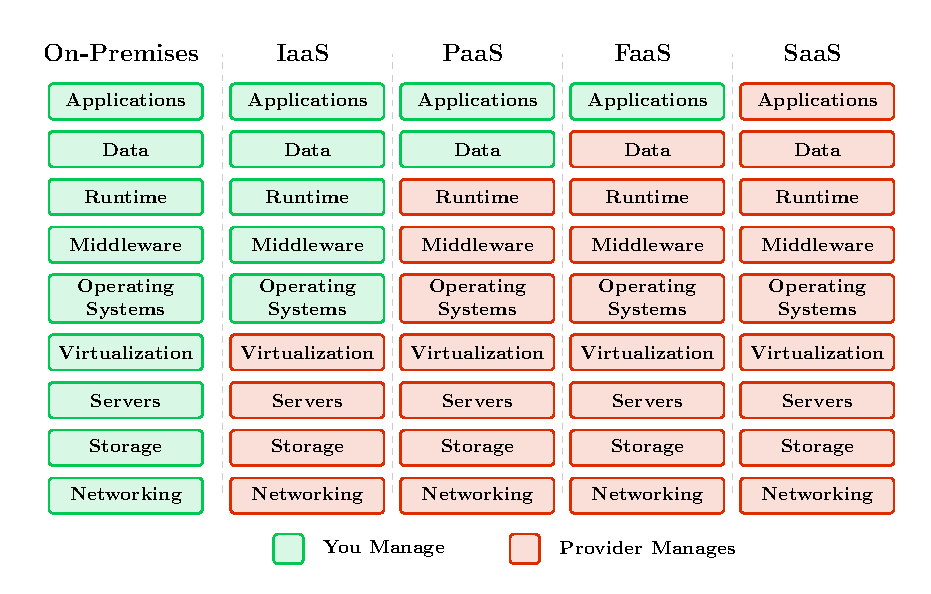
\includegraphics[width=0.8\textwidth]{figures/iaas_paas_faas_saas.pdf}
    \caption{The Shared Responsibility Model across varying Cloud Computing Paradigms.}
    \label{fig:iaas_paas_faas_saas}
\end{figure}

For the purposes of this research, SaaS falls outside the scope of architectural implementation. The critical transition lies between PaaS and FaaS. The relentless industry drive toward rapid elasticity, microsecond billing, and extreme resource efficiency in FaaS and edge environments exposed the limitations of traditional, heavy deployment artifacts. Developers pushing code to serverless platforms require instantaneous execution. Standard OCI containers, laden with operating system userlands, introduce severe latency bottlenecks in these paradigms, necessitating a shift toward the lightweight isolation models that WebAssembly provides.

\subsection{Microservice Architecture}
Microservice architecture emerged as the logical software design pattern for cloud-native deployment. Unlike traditional monolithic applications—where all business logic, user interfaces, and database connections are tightly coupled into a single executable—microservices decompose an application into a collection of small, independently deployable, and loosely coupled services that communicate over a network via language-agnostic APIs ~\cite{newman2015building}.

This paradigm offers distinct advantages: development agility, localized fault isolation, and the ability to scale specific system bottlenecks independently. However, it introduces severe distributed system challenges. Managing network latency, data consistency, and the operational overhead of packaging and deploying hundreds of individual services necessitated the creation of entirely new virtualization and orchestration layers.

\section{Containerization and Orchestration}
\label{sec:containerization}

\subsection{Virtual Machines vs. Containers}
To solve the deployment complexity of microservices, the industry initially relied on Virtual Machines. However, VMs require a hypervisor to emulate physical hardware, atop which a complete guest OS is installed. This results in gigabytes of memory overhead and startup times measured in minutes, making them inherently unsuitable for transient, rapidly scaling microservices.

Docker revolutionized the landscape by democratizing Linux containers. Instead of virtualizing the hardware, containers virtualize the operating system ~\cite{merkel2014docker}. Docker relies on two core Linux kernel features:
\begin{enumerate}
    \item \textbf{Namespaces:} Provide process isolation, ensuring the container has its own isolated filesystem, network interfaces, and process tree.
    \item \textbf{Cgroups (Control Groups):} Limit, isolate, and monitor the resource usage (CPU, memory, disk I/O) of a given process.
\end{enumerate}

\begin{figure}[htbp]
    \centering
    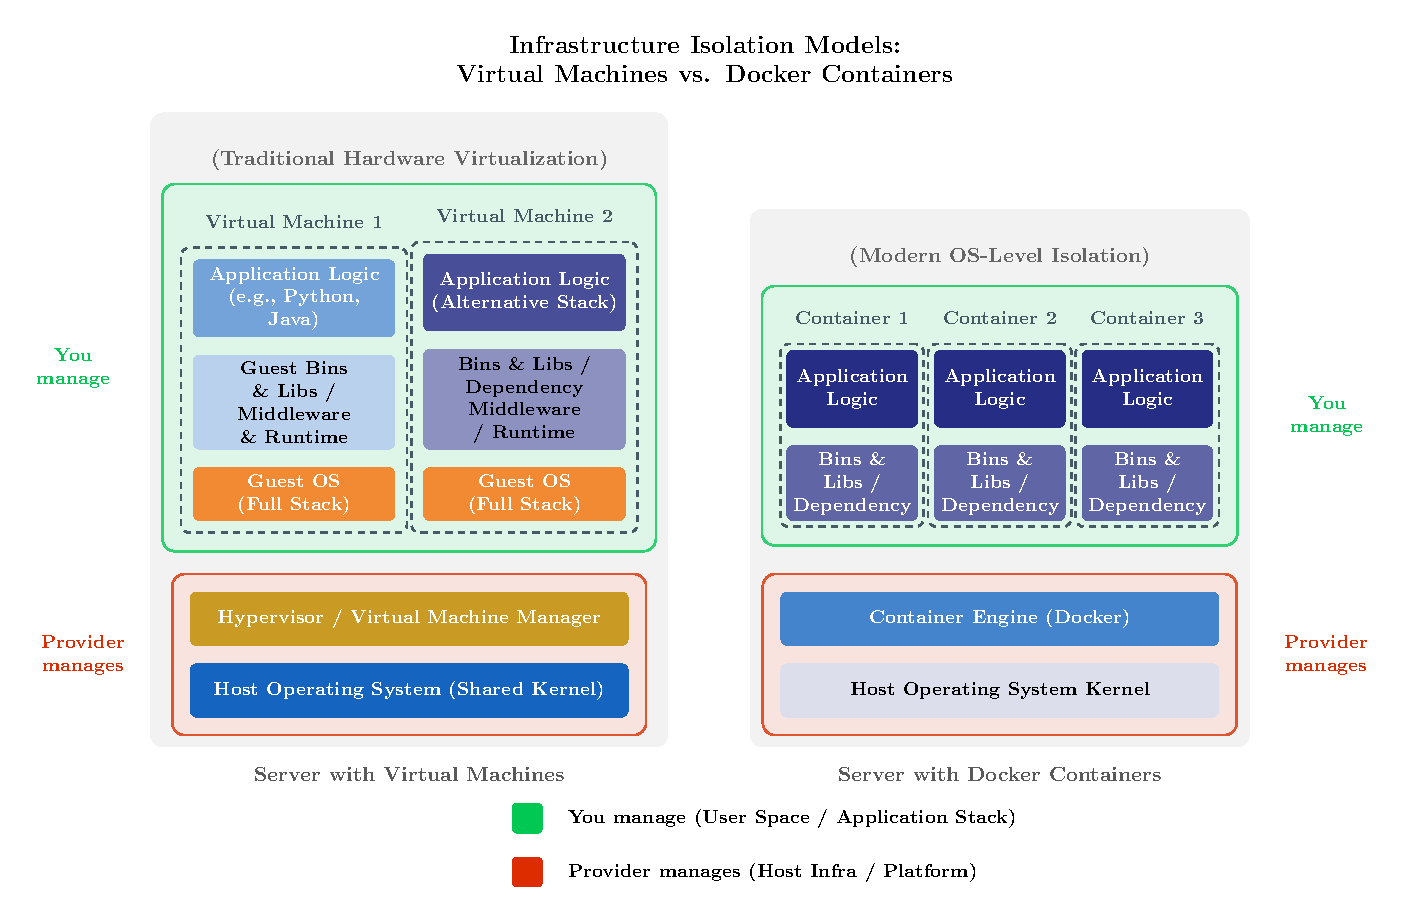
\includegraphics[width=\textwidth]{figures/virtual_machine_vs_docker.pdf}
    \caption{Infrastructure Isolation Models: Virtual Machines vs. Docker Containers}
    \label{fig:virtual_machine_vs_docker}
\end{figure}

Docker’s definitive innovation was the standardization of the container image format, now governed by the Open Container Initiative (OCI). By packaging application code alongside its dependencies, libraries, and a base filesystem into a single portable unit, Docker ensured environment consistency from a developer's laptop to production servers.

Despite its dominance, the OCI standard has inherent drawbacks. Because containers share the host's Linux kernel, a kernel-level vulnerability can potentially compromise all containers on that host, posing security risks in multi-tenant environments. Furthermore, traditional container images are bulky; they bundle a userland OS and language runtimes alongside the application. This bulk introduces latency during image transfer and initialization—known as the "cold start" problem—which is highly detrimental in FaaS and edge computing environments ~\cite{gadepalli2020challenges}.

\subsection{Kubernetes Orchestration}
As microservices proliferated, manually managing individual containers across a fleet of servers became operationally unfeasible. Kubernetes emerged as the industry-standard container orchestration platform. It abstracts the underlying cluster of hardware, allowing engineers to declare the desired state of their applications rather than manually scripting deployments ~\cite{burns2016borg}.

Kubernetes operates on a distributed architecture. The Control Plane dictates instructions to worker nodes. Each worker node runs an agent called a Kubelet, which manages Pods—the smallest deployable computing unit, typically containing one or more tightly coupled containers. Crucially, Kubernetes communicates with the underlying container runtime (like containerd or CRI-O) via the Container Runtime Interface (CRI). This decoupled architecture established strict standardizations, eventually allowing alternative, non-Linux execution environments, such as WebAssembly, to be orchestrated seamlessly alongside standard OCI-compliant containers.

\begin{figure}[htbp]
    \centering
    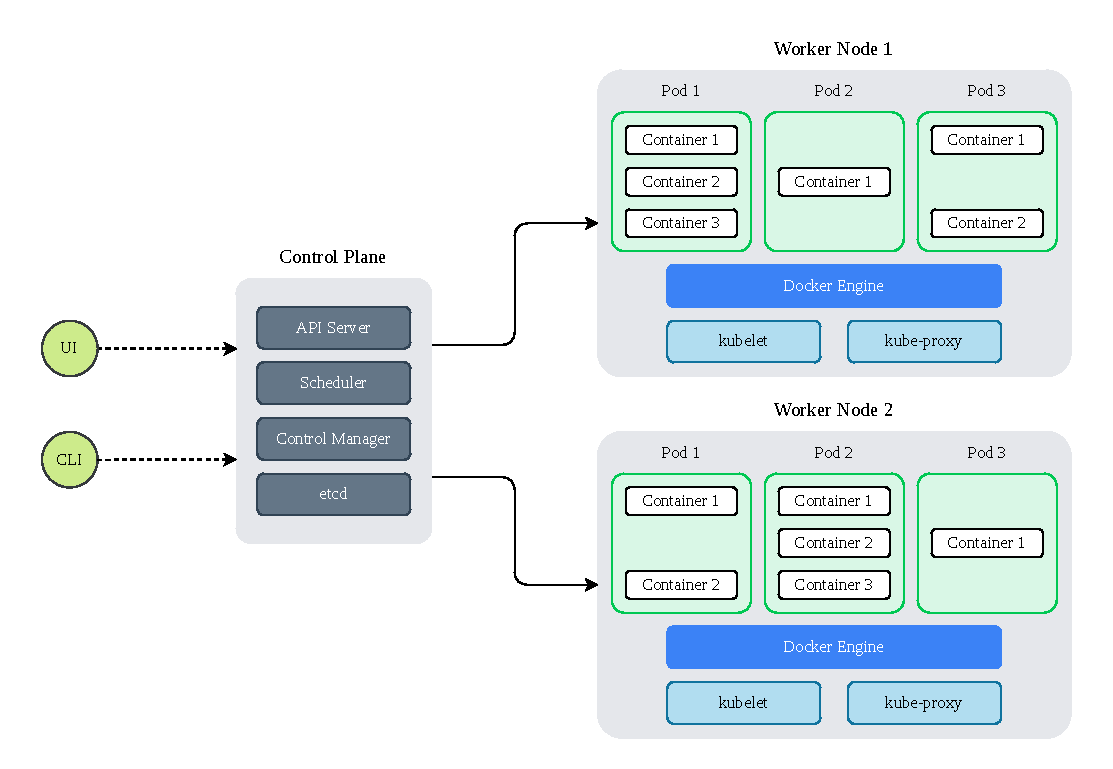
\includegraphics[width=0.8\textwidth]{figures/k8s_architecture.pdf}
    \caption{Kubernetes Architecture}
    \label{fig:kubernetes_architecture}
\end{figure}

\section{WebAssembly (Wasm)}
\label{sec:wasm}

\subsection{Origin and Technical Architecture}
WebAssembly (Wasm) is a binary instruction format designed for a stack-based virtual machine. It originated from the need to execute high-performance code within web browsers—a domain historically constrained by JavaScript's inconsistent performance and parsing overhead. WebAssembly was officially released in 2017 as a W3C standard, sitting alongside HTML, CSS, and JavaScript as an official language of the web ~\cite{haas2017bringing}.

Wasm functions as an agnostic hardware abstraction layer. Developers write code in systems languages like C, C++, or Rust, and compile it down to \texttt{.wasm} binaries. 

\begin{figure}[htbp]
    \centering
    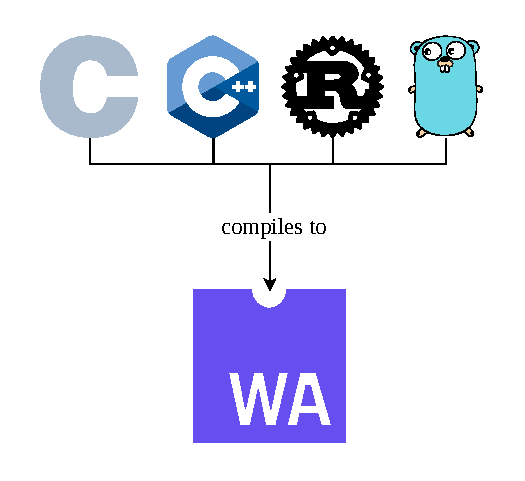
\includegraphics[width=0.5\textwidth]{figures/languages_compile_to_wasm.pdf}
    \caption{Compiling different languages to Wasm}
    \label{fig:compiling_different_langauges_to_wasm}
\end{figure}

\subsection{Module Structure and Stack-Based Execution}
WebAssembly is fundamentally a stack machine. Unlike register-based physical CPU architectures (such as x86\_64 or ARM64), Wasm instructions implicitly operate on an operand stack. Variables are pushed onto the stack, and operations pop these operands, compute the result, and push it back.  This design yields highly compact binary modules, as instructions do not need to explicitly encode register numbers, accelerating both transmission over networks and decoding phases.

A Wasm application is distributed as a strictly standardized binary module consisting of discrete sections. These include the Type section (function signatures), Import section (host-provided dependencies), Code section (executable bytecode), and Data section (initial memory state). Before execution, a WebAssembly runtime performs a deterministic, single-pass validation to ensure type safety and structural integrity. Because the bytecode is designed to map cleanly to native machine instructions, runtimes employ Just-In-Time (JIT) or Ahead-Of-Time (AOT) compilation engines (such as Cranelift or LLVM) to translate Wasm into highly optimized, native machine code instantaneously.

\subsection{Memory Management and Isolation}
One of WebAssembly's defining technical characteristics is its approach to memory management and fault isolation.  The architecture relies on the following core principles:
\begin{itemize}
    \item \textbf{Compact Binary Format:} The \texttt{.wasm} format is highly optimized, allowing for rapid fetching, decoding, and execution.
    \item \textbf{Hardware Agnosticism:} Because it utilizes a virtual stack machine, the compiled bytecode makes no assumptions about the underlying physical CPU architecture, enabling true portability across varied cloud node pools.
    \item \textbf{Linear Memory Space:} Wasm operates in a contiguous, resizable array of bytes known as linear memory. Code executing within the Wasm module operates strictly with integer offsets within this array; it cannot execute arbitrary pointers or access host memory outside this strictly enforced boundary.
    \item \textbf{Software-Based Fault Isolation (SFI):} Unlike Docker, which relies on the host OS kernel (cgroups/namespaces) to contain a process, Wasm achieves isolation mathematically at the runtime level. Any attempt to access memory outside the allocated linear boundary results in a deterministic trap, halting the module instantly without compromising the host.
\end{itemize}

\subsection{Language Agnosticism and the JVM Comparison}
The concept of "Write Once, Run Anywhere" (WORA) was popularized by Java. Java achieves portability by compiling source code to Java bytecode, which is executed by the Java Virtual Machine (JVM). However, WebAssembly fundamentally differs from the JVM in design and scope. The JVM was built specifically to execute Java and inherently carries a heavyweight runtime featuring built-in garbage collection. Conversely, Wasm was designed as a low-level, truly language-agnostic compilation target without an opinionated runtime, making it exceptionally lightweight. 

\begin{figure}[htbp]
    \centering
    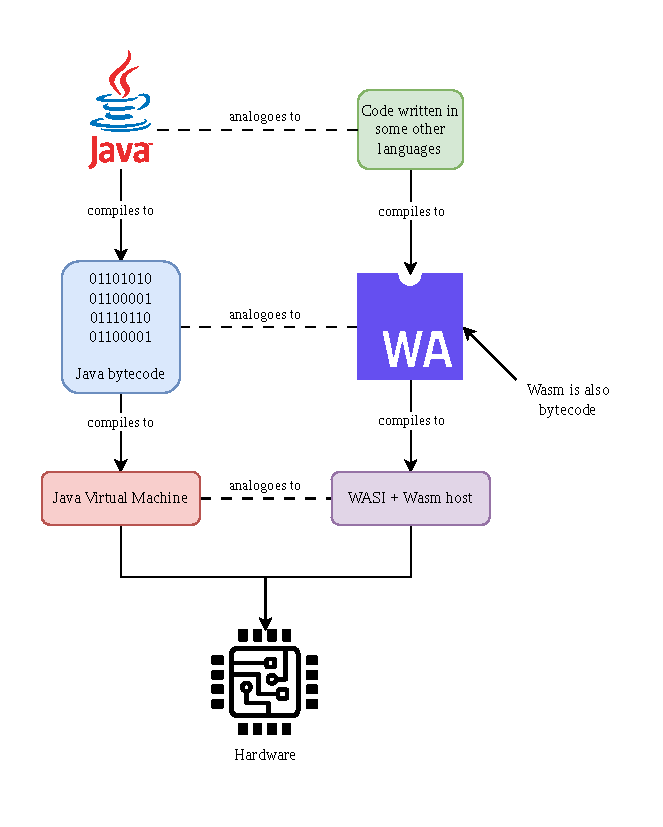
\includegraphics[width=0.7\textwidth]{figures/java_vs_wasm.pdf}
    \caption{An analogy comparing the cross-platform execution models of Java and WebAssembly. Adapted from Chiarlone \cite{chiarlone2024serverside}.}
    \label{fig:java_vs_wasm}
\end{figure}

For languages requiring automatic memory management (like Go, Python, Kotlin, or PHP), Wasm historically required the entire language runtime and garbage collector to be compiled and bundled inside the \texttt{.wasm} binary. This approach bloated the deployment artifact and created redundant layers of memory management. For instance, deploying a compiled-to-Wasm language with its own garbage collector into a host environment that already possesses one (such as a browser engine like V8) is highly wasteful \cite{steiner2023wasmgc}. Furthermore, having no interaction between Wasm's linear memory and the built-on-top garbage collector of the ported language often caused problems like memory leaks and inefficient collection attempts \cite{liedtke2023v8wasmgc}.

To resolve this, the WebAssembly Garbage Collection (WasmGC) standard has been introduced to delegate memory management directly to the host environment. WasmGC extends the WebAssembly memory model by adding struct and array heap types, thereby providing native support for non-linear memory allocation \cite{wasm2023gcproposal}. Because each WasmGC object has a fixed type and structure, host VMs can generate highly efficient access code without the risk of dynamic deoptimizations. This allows higher-level managed languages to bypass bundling their own garbage collectors, instead interfacing efficiently with the host VM's built-in garbage collector.

The architectural impact on artifact density is significant. By eliminating the need to bundle memory management code, WasmGC binaries for managed languages can achieve dramatically smaller footprints. In early benchmarks, WasmGC binaries for languages like Java were proven to be considerably smaller than equivalent modules compiled from C or Rust, because C and Rust must still bundle manual memory management routines like \texttt{malloc} and \texttt{free} inside the binary \cite{steiner2023wasmgc}. This advancement firmly positions Wasm as a viable, high-density target for the entire spectrum of modern programming languages.

\subsection{The Server-Side Evolution: WASI}
While Wasm successfully delivered near-native performance for computationally heavy browser applications, its portability, mathematical security model, and minimal footprint rapidly garnered interest for backend deployment. Solomon Hykes, the founder of Docker, once famously stated: 
\begin{quote}
    If WASM+WASI existed in 2008, we wouldn't have needed to create Docker. That's how important it is. WebAssembly on the server is the future of computing. ~\cite{hykes2019tweet}
\end{quote}
 
Because Wasm is entirely isolated by default, a bare Wasm module running on a server cannot open a network socket, read a file, or query the system clock. In 2019, the WebAssembly System Interface (WASI) was introduced to solve this. WASI defines a standardized API specification that provides Wasm modules with secure, granular, capability-based access to the host operating system ~\cite{clark2019standardizing}. By acting as a secure POSIX-like layer, WASI transforms Wasm from a sandboxed browser calculator into a fully functional server-side technology.

\subsection{Capability-Based Security Model}
WASI implements a capability-based security model that diverges significantly from traditional Linux permissions.  A Linux container limits an already-running OS environment. WASI, however, enforces a strict "deny-by-default" posture. 

If a Wasm module needs to access a configuration file, it cannot invoke a standard `open()` system call for an arbitrary path (e.g., `/etc/config`). Instead, the host runtime must explicitly grant the module a "pre-opened" file descriptor at startup. The module is completely blind to the existence of the host filesystem outside the specific directory tree explicitly mapped and passed to it by the runtime.

\begin{figure}[htbp]
    \centering
    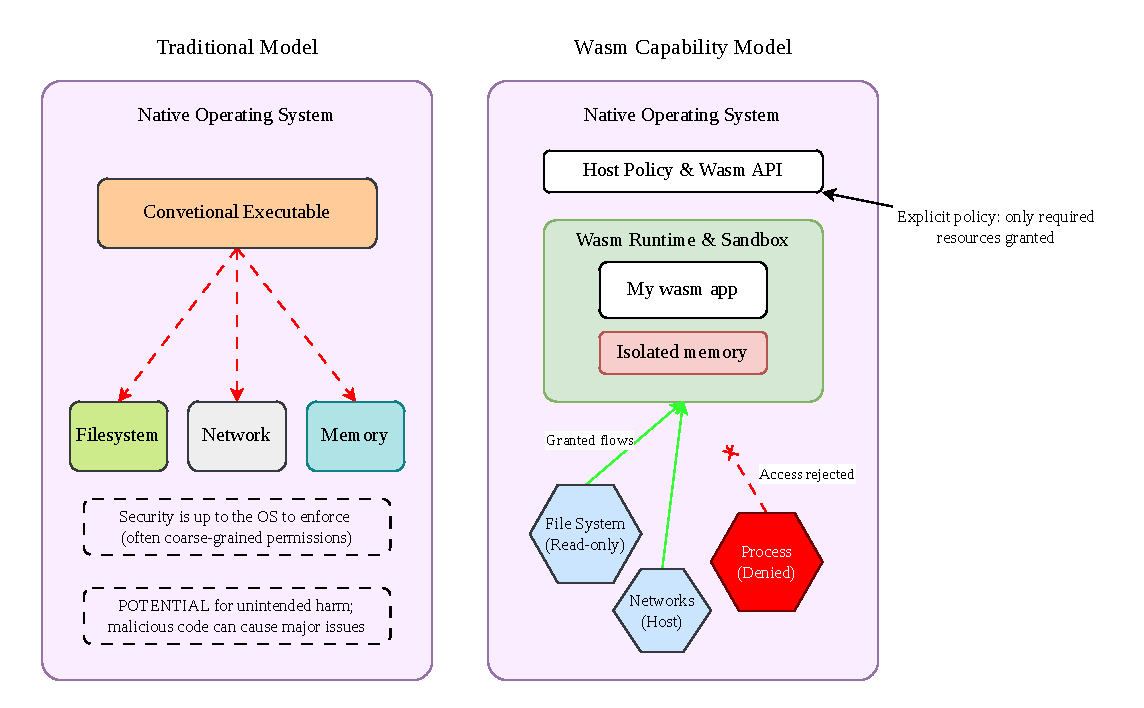
\includegraphics[width=\textwidth]{figures/wasm_sandboxed_model.pdf}
    \caption{Comparative Security Models: Traditional vs Wasm Capabilities}
    \label{fig:wasm_sandboxed_model}
\end{figure}

\subsection{Architectural Evolution: From POSIX to the Component Model}
The initial iteration of WASI (often referred to as WASI Preview 1) was heavily modeled after standard POSIX interfaces, focusing on file descriptors, environment variables, and standard I/O streams. While effective for simple command-line tools and basic microservices, this POSIX-centric approach introduced friction when handling complex, multi-language cloud-native interactions.

To address this, the WebAssembly ecosystem is currently transitioning to the WebAssembly Component Model (WASI Preview 2 and Preview 3).  The Component Model shifts WASI from a low-level POSIX API to a high-level, language-agnostic interface system utilizing WebAssembly Interface Types (WIT). This advancement allows discrete Wasm components—potentially written in entirely different source languages—to natively interoperate. They can securely pass complex data types (such as strings, records, and variants) across execution boundaries without sharing linear memory, laying the foundation for highly modular, secure, and dynamically composable microservice architectures.

\subsection{Wasm vs. Traditional Containers}
Applying Wasm and WASI to the server yields a deployment artifact that sits functionally between a traditional VM and an OCI container, offering unique operational characteristics:

\begin{enumerate}
    \item \textbf{Cold Start and Footprint:} Traditional OCI containers bundle an OS userland, frequently resulting in image sizes exceeding 100MB and startup times measured in seconds. A Wasm module contains only the compiled application logic. Wasm binaries are typically just a few megabytes and can be instantiated by a host runtime in microseconds. Long et al. demonstrated that Wasm runtimes can perform at least 10x faster than Docker from a cold start for short-running workloads ~\cite{long2023wasm}. Hall and Ramachandran further verified that Wasm's improved cold start times lead to up to 90\% faster response times for basic serverless tasks ~\cite{hall2021serverless}.
    \item \textbf{Security and Density:} Wasm utilizes Software-Based Fault Isolation (SFI). If a Wasm module is compromised, the attacker only controls the isolated linear memory sandbox. Because Wasm threads do not require full OS process overhead, the minimal memory footprint allows Kubernetes nodes to achieve exponentially higher workload density.
    \item \textbf{Performance Trade-offs:} Despite its advantages in density and initialization, Wasm remains structurally immature compared to Docker regarding concurrency. Wasm currently lacks robust, standardized multithreading capabilities (the Wasm Threads proposal relies on shared memory buffers that complicate isolation). Sondell (2024) demonstrated that in high-concurrency HTTP server scenarios, a Docker container can process requests significantly faster because it can scale natively across multiple CPU cores, whereas a single Wasm instance frequently remains bottlenecked by single-threaded execution ~\cite{sondell2024performance}. Furthermore, Spies and Mock found that single-threaded Wasm apps perform approximately 14\% slower than native x86\_64 binaries due to sandbox bounds-checking overhead ~\cite{spies2021evaluation}.
\end{enumerate}

By utilizing WASI shims (such as \texttt{runwasi}), Kubernetes can now orchestrate these high-density Wasm workloads directly alongside traditional Docker containers, establishing the precise technological foundation for the comparative analysis executed in this research.